\documentclass[11pt,a4paper]{article}
\usepackage[a4paper,margin=2.3cm]{geometry}
\usepackage[T1]{fontenc}
\usepackage[utf8]{inputenc}
\usepackage{lmodern}
\usepackage{microtype}
\usepackage{amsmath,amssymb,bm}
\usepackage{graphicx}
\usepackage{booktabs}
\usepackage{array}
\usepackage{caption}
\usepackage{subcaption}
\usepackage{xcolor}
\usepackage{enumitem}
\usepackage{natbib}
\usepackage[hidelinks]{hyperref}
\usepackage{float}
\usepackage{adjustbox}
\newcommand{\fittable}[1]{\begin{adjustbox}{max width=\textwidth}\input{#1}\end{adjustbox}}
\captionsetup{font=small,labelfont=bf}
\setlist{nosep,leftmargin=1.4em}
\setlength{\parskip}{0.35em}
\setlength{\parindent}{0pt}
\graphicspath{{../results/figures/}}
\newcommand{\tabdir}{../results/tables}
\newcommand{\E}{\mathbb{E}}
\newcommand{\1}{\mathbf{1}}

\title{\textbf{FuelGuard}: forecasting volatility with machine learning\\
to hedge diesel costs for small Italian hauliers}
\author{{[Member 1]} \quad {[Member 2]} \quad {[Member 3]} \quad {[Member 4]} \quad {[Member 5]}\\[0.4em]
\small Introduction to Machine Learning -- Group project\\
\small MSc in Financial Engineering, EDHEC Business School}
\date{2 December 2026}

\begin{document}
\maketitle
\begin{abstract}
\noindent Small Italian hauliers spend around 30\% of their costs on diesel and cannot absorb shocks such
as the +32\% monthly jump of March 2022. FuelGuard is a monthly signal, offered by a bank to its SME transport
clients, that forecasts next month's diesel volatility and turns it into a hedge ratio and a 95\%
worst-case cost. A first attempt to predict price spikes directly showed that the direction of diesel prices is
essentially unpredictable; following the volatility-forecasting literature, FuelGuard~2.0 forecasts
\emph{risk} instead. We train Lasso, random forests, gradient boosting and a neural network on a panel of 22
futures markets (Bloomberg, 2007--2026, 109\,000 market-days, 30 features including the implied-volatility
smile) and compare them, in a purged walk-forward over 15 test years, with the random walk, HAR and HAR with
implied volatility (HAR-IV). Machine learning alone matches but does not beat HAR-IV; the combination of
HAR-IV with a scale-free ML ensemble, chosen on a separate validation period, reduces the forecast error by
2.3\% (Diebold--Mariano $p<0.001$), by 26\% against HAR and by 37\% against the random walk, and improves
on HAR-IV in 20 of 22 markets and 13 of 15 years. For diesel, volatility-driven hedging cuts the average cost
of the worst 5\% of months from 16.7\% to 6.6\% above the lockable price while lowering the average cost.
\end{abstract}

\section{The product}\label{sec:product}

\paragraph{Who uses it.} Road haulage in Italy is dominated by very small firms: the typical
\emph{autotrasportatore} runs a handful of trucks. Diesel is one of their largest costs, typically around
30\% of operating costs, and their margins are a few percent of revenue. A ten-truck firm burns about
25\,000 litres a month; in our data the wholesale price rose by 32\% in a single month in March 2022
(about 5\,000~EUR on a month's fuel bill) and by 60\% in March 2026. These firms do not trade futures, but
they can ask their fuel supplier or their bank for a fixed price for next month. The question they cannot
answer is \emph{when} fixing is worth its cost (we assume a 1\% margin over the futures price).

\paragraph{The client.} We pitch FuelGuard to a \textbf{bank with SME loans to transport firms}. Fuel
shocks are a credit-risk driver for these borrowers, and the bank can sell fixed-price fuel or simple
swaps. Each month FuelGuard gives the bank, for each client, two numbers it can pass on through its
relationship managers or app:
\begin{enumerate}
\item a \textbf{hedge ratio} (0\%, 50\% or 100\% of next month's diesel), and
\item a \textbf{95\% worst case}: ``next month, there is a 5\% chance that your diesel will cost more than
X\% above the price you can fix today''.
\end{enumerate}

\paragraph{The prediction.} Both numbers come from one machine-learning task: a \textbf{regression of next
month's realised volatility} of diesel futures. Our first design tried to predict the price itself, or
whether it would jump by more than 5\%. Out of sample, the size of next month's price move could not be
predicted beyond the futures price, and the modest skill in predicting jumps came almost entirely from
implied volatility (Appendix~\ref{app:v1}). Following the literature, which finds that volatility is
persistent and predictable while price changes are not \citep{corsi2009,christensen2023,degiannakis2017},
FuelGuard~2.0 forecasts \emph{how much} the price will move, not in which direction. For a hedger this is
the relevant quantity: the risk of a costly month grows with volatility.

\paragraph{What it replaces (benchmarks).} The haulier's current practice (never fix, always fix, fix half)
for the decision; and, for the forecast, the three models a risk desk would use today: last month's
volatility (random walk), the HAR model of \citet{corsi2009}, and HAR augmented with the option-implied
volatility (HAR-IV), the market's own forecast. HAR-IV is the bar the machine-learning models must clear.

\section{Data}\label{sec:data}

\paragraph{Sources, period, unit.} The core dataset is a \textbf{panel of 22 futures markets} downloaded
from Bloomberg, daily from January 2007 to November 2026 (Table~\ref{tab:markets} in
Appendix~\ref{app:data}): four energy contracts (NY Harbor diesel, Brent, WTI, natural gas), three metals,
three grains, three softs, two livestock contracts and seven US and German government-bond futures. For each
market and day we have the open, high, low and settlement price, volume, the second-month price, and the
30-day implied volatility at seven strikes (90\% to 110\% of the forward) plus the first- and second-month
at-the-money volatility; three common series (VIX, 3-month VIX, VSTOXX) complete the set: \textbf{15 raw
variables per market plus 3 common ones}. The unit of observation is a \textbf{market-day}; after the
first month of history needed by the realised-volatility features and dropping the last month (outcome
unknown), the sample has \textbf{109\,332 market-days} (about 5\,000 per market; features with longer
windows are missing at the start and are imputed or handled natively by the models). For the hedging application we reuse the diesel
cost in euros per litre, built from the diesel futures and the ECB EUR/USD rate (Appendix~\ref{app:v1}).

\paragraph{Target: next month's realised volatility.} For each market and day $t$ we compute the
Garman--Klass variance $\hat\sigma^2_{GK,s}=\tfrac12\ln^2(H_s/L_s)-(2\ln2-1)\ln^2(C_s/O_s)$ from the open,
high, low and settlement of the same contract on the same day \citep{garman1980}, and the target is
\[ y_t=\ln\sqrt{252\cdot\tfrac{1}{21}\textstyle\sum_{s=t+1}^{t+21}\hat\sigma^2_{GK,s}} ,\]
the log annualised volatility over the next 21 trading days. Two reasons for this choice: range-based
estimators are far less noisy than squared returns \citep{alizadeh2002}, and, because they never compare
prices of two different contracts, they are immune to the jumps of generic futures series at contract rolls.
Median volatility ranges from 0.8\% (Euro Schatz) to 44\% (natural gas); diesel's is 27.5\%
(Figure~\ref{fig:diesel}).

\paragraph{Features (30, in nine groups).} All are computed from data up to the close of $t$:
(i) \emph{HAR terms}: log realised volatility over 1, 5, 22 and 63 days;
(ii) \emph{implied-volatility level} and its 5- and 22-day changes;
(iii) the \emph{variance risk premium}, log implied minus log realised volatility;
(iv) the \emph{smile}: skew $(\sigma_{90}-\sigma_{110})/\sigma_{100}$ and the put and call wings;
(v) the implied-volatility \emph{term structure} (2nd vs 1st month);
(vi) \emph{returns and asymmetry}: the 22-day intraday return, the share of ``bad'' (downside) variance
\citep{pattonsheppard2015} and the frequency of jump days;
(vii) \emph{volume} relative to its 3-month median and the futures-curve slope;
(viii) \emph{common risk}: VIX, VIX term structure, VSTOXX and the 5-day change of VIX;
(ix) the market's long-run volatility, the month, and asset-class indicators.

\paragraph{Preparation.} Days with non-positive prices (WTI, April 2020) are dropped; ranges above 40\% in a
day are capped as data errors; implied volatilities below a third or above three times their own past
three-month median are treated as missing and carried forward for at most five days (all backward-looking);
common series are aligned forward only. Because ML models pool 22 markets whose volatility differs by a
factor of 50, they use \emph{scale-free} inputs: every log-volatility level is expressed relative to the
market's current 22-day level, which itself is expressed relative to the market's long-run average, and the
ML target is the \emph{change} $y_t-\ln\sigma^{(22)}_t$ (Section~\ref{sec:methods}). An automated test
scrambles all prices after a date and checks that no feature before it changes.

\begin{figure}[t]
\centering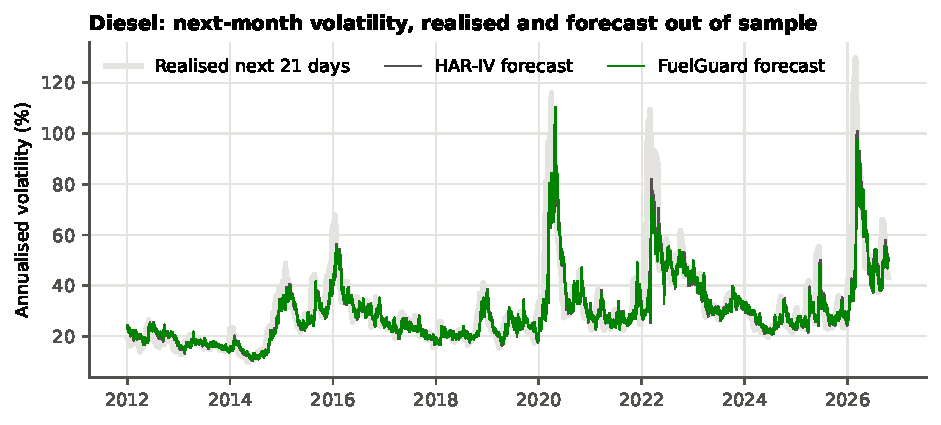
\includegraphics[width=\textwidth]{v2_fig_diesel_forecast.pdf}
\caption{Diesel: realised volatility over the next 21 trading days (grey) and two out-of-sample forecasts
made at the start of the window, 2012--2026.}
\label{fig:diesel}
\end{figure}

\section{Methods}\label{sec:methods}

\paragraph{Learning problem.} We estimate $m(x_{it})=\E[y_{it}\mid x_{it}]$ for market $i$ and day $t$
by minimising the squared error of the log volatility, a loss that ranks volatility forecasts consistently
even though realised volatility is only a noisy proxy of the true one \citep{patton2011}.

\paragraph{Benchmarks (what the product must beat).} (1) \emph{Random walk}: next month's volatility equals
the last month's. (2) \emph{HAR} \citep{corsi2009}, estimated by OLS separately for each market on its
training window: $y_{it}=\beta_{0i}+\beta_{di}\ln\sigma^{(1)}_{it}+\beta_{wi}\ln\sigma^{(5)}_{it}
+\beta_{mi}\ln\sigma^{(22)}_{it}+\varepsilon_{it}$, the standard benchmark of the volatility literature.
(3) \emph{HAR-IV}: HAR plus the log implied volatility, the market's own forecast. HAR-IV is linear, has five
parameters per market and is very hard to beat; it assumes that the relation between past, implied and
future volatility is linear in logs and stable within each market.

\paragraph{Machine-learning models (pooled across the 22 markets).} Pooling multiplies the sample by 22
and lets a model learn patterns common to all futures markets \citep{gu2020}, at the price of
heterogeneity, which the scale-free inputs remove. All models predict the change in log volatility.
\begin{itemize}
\item \textbf{Lasso}: linear in the 30 features with an $L_1$ penalty $\alpha\in\{10^{-4},10^{-3},10^{-2}\}$,
which selects variables. Assumes linearity and additivity; needs standardised inputs.
\item \textbf{Random forest}: 300 trees on 50\% subsamples with a third of the features tried at each split;
depth $\{6,12\}$, minimum leaf $\{20,100\}$. Captures non-linearities and interactions (e.g.\ a high variance
risk premium matters more when VIX is high); no extrapolation beyond the training range.
\item \textbf{Gradient boosting}: shallow trees fitted sequentially to the residuals, learning rate 0.05;
number of trees $\{200,500\}$, depth $\{3,5\}$.
\item \textbf{Neural network}: a two-layer perceptron (64 and 32 ReLU units), Adam, early stopping, weight
penalty $\alpha\in\{10^{-4},10^{-2}\}$; the most flexible model and the one that needs the most data.
\item \textbf{ML ensemble}: the equal-weight mean of Lasso, random forest and boosting.
\item \textbf{FuelGuard} (the product): the equal-weight mean of HAR-IV and the ML ensemble, combining an
econometric model that knows each market's level with ML models that learn common non-linear dynamics.
\end{itemize}
Appendix~\ref{app:theory} explains each method and its assumptions.

\paragraph{How the design was chosen.} A first run with ML models on raw (not scale-free) features lost to
HAR-IV. To change the design \emph{without} looking at the test years, we compared alternatives on a separate
\textbf{validation period, 2010--2011}, using only labels known before December 2009
(\texttt{scripts/10\_validation\_design.py}, Table~\ref{tab:design} in Appendix~\ref{app:additional}). There,
scale-free inputs beat raw ones for every model (e.g.\ random forest $-25\%\to-2\%$ against HAR-IV), the
neural network overfitted in every variant (so it is reported but not in the ensemble), and combining the ML
ensemble with HAR-IV gave the lowest error ($+4.5\%$). These choices were then frozen.

\section{Evaluation design}\label{sec:evaluation}

\paragraph{Walk-forward with purging and embargo.} For each test year $Y=2012,\dots,2026$, every model is
re-estimated on all market-days whose 21-day label is fully observed at least 30 calendar days before
1~January of $Y$, and then forecasts every market-day of $Y$: 15 test years and \textbf{80\,224
out-of-sample market-days} (3\,724 for diesel), covering the 2014--16 oil crash, Covid, the 2022 energy crisis
and 2026. HAR and HAR-IV are re-estimated per market on all training days. The ML models train on every fifth
day of each market (labels overlap over 21 days, so consecutive days add little information; this also
divides the cost by five) and choose their hyper-parameters by a three-fold \emph{purged} cross-validation
inside the training window (the most recent 15\% blocks of dates, with the same 30-day gap). Automated tests
check that training labels end before the test year and that features never use future prices
(Appendix~\ref{app:theory}, A.6).

\paragraph{Statistical metrics.} Mean squared error of the log volatility and QLIKE \citep{patton2011};
the out-of-sample $R^2$ relative to a benchmark $b$, $R^2_{OS}=1-\sum(y-\hat y)^2/\sum(y-\hat y_b)^2$
(positive values mean the model beats $b$); and Diebold--Mariano tests against HAR-IV. For the pooled test we
average the loss differential across markets each day and use Newey--West errors with 21 lags; we also test
each market separately.

\paragraph{From volatility to the hedging decision.} The haulier gets two numbers each month:
\begin{enumerate}
\item \textbf{A hedge ratio.} On the first trading day of each month, FuelGuard locks 100\% of next month's
diesel if forecast volatility is above the 75th percentile of diesel's historical volatility, 50\% if it is
above the median, and 0\% otherwise; both percentiles use data before the test year only. The same rule is
applied to every forecast, so differences come from the forecast alone. Costs are measured as in
Appendix~\ref{app:v1}: overrun $c_t/P_t-1$ of the monthly cost over the price lockable at decision time,
with a 1\% hedging margin, 178 monthly decisions from January 2012 to October 2026.
\item \textbf{A 95\% worst case.} If prices follow a random walk with forecast volatility $\hat\sigma$, the
premium of the monthly average price over the price locked at $t+1$ has standard deviation
$\hat\sigma\sqrt{(n+1)(2n+1)/(6n)/252}$ with $n=21$, about $\hat\sigma\sqrt{7.5/252}$. The 95\% bound is
$1.645$ times this. We count how often the realised premium exceeds it (5\% expected) and apply the
\citet{kupiec1995} test.
\end{enumerate}

\section{Results}\label{sec:results}

\subsection{Forecast accuracy}

\begin{table}[H]
\centering\small
\fittable{\tabdir/vol_pooled.tex}
\caption{Out-of-sample accuracy, 22 markets, 2012--2026 (80\,224 market-days). Loss: squared error of log
volatility; $R^2$ vs a benchmark is the reduction of its MSE. DM: Diebold--Mariano statistic against
HAR-IV on the daily cross-market average loss (Newey--West, 21 lags); negative values favour the model.}
\label{tab:pooled}
\end{table}

\paragraph{Volatility is predictable.} Table~\ref{tab:pooled} shows that forecasting volatility is a very
different problem from forecasting prices. Every model except the neural network improves on the random
walk by 34--37\%, and within each market the forecasts explain most of the variation of next month's
volatility (e.g.\ $R^2=74\%$ for diesel, Table~\ref{tab:diesel}). Option prices carry the most information:
adding implied volatility to HAR (HAR-IV) reduces the error by 24\% relative to HAR.

\paragraph{Machine learning alone matches HAR-IV; combined with it, it beats it.} The three tree and
linear ML models are within 1.6--2.4\% of HAR-IV and the difference is not significant; their ensemble is
statistically indistinguishable from HAR-IV ($-0.2\%$, $p=0.89$). The neural network is 31\% worse: even
with 20\,000 training rows and early stopping it overfits, as the validation period had shown. The product,
the equal-weight combination of HAR-IV and the ML ensemble, \textbf{reduces the error by 2.3\% relative to
HAR-IV} with a Diebold--Mariano statistic of $-4.8$ ($p<0.001$), also improves the QLIKE loss, and beats
HAR-IV in 13 of the 15 test years (Appendix~\ref{app:additional}). A 2\% gain over HAR-IV is in line with
the gains reported by \citet{christensen2023} for individual stocks. The combination works because HAR-IV and
the ML models make different errors: HAR-IV is market-specific and linear, the ML ensemble is pooled and
non-linear.

\begin{figure}[t]
\centering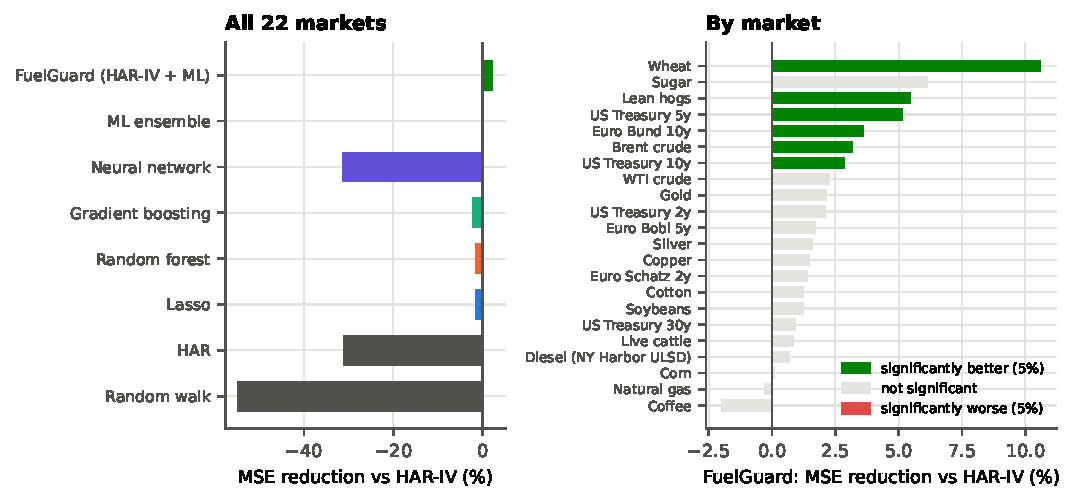
\includegraphics[width=\textwidth]{v2_fig_accuracy.pdf}
\caption{Left: MSE reduction against HAR-IV, all markets. Right: FuelGuard against HAR-IV by market; colour
indicates a Diebold--Mariano test at 5\%.}
\label{fig:accuracy}
\end{figure}

\paragraph{By market.} FuelGuard improves on HAR-IV in 20 of 22 markets, significantly in six (wheat, lean
hogs, Brent and three government bonds), and is never significantly worse (Figure~\ref{fig:accuracy}).
Gains are largest for wheat, sugar and lean hogs. For energy as a group the gain is
1.7\% ($p=0.04$); for diesel alone it is 0.7\% and not significant (Table~\ref{tab:diesel}): on its own
product, FuelGuard is as good as the best econometric benchmark, not clearly better.

\begin{table}[H]
\centering\small
\fittable{\tabdir/vol_diesel.tex}
\caption{Diesel (NY Harbor ULSD) only, 3\,724 out-of-sample days. DM test per market, Newey--West 21 lags.}
\label{tab:diesel}
\end{table}

\paragraph{What drives the forecasts.} Shuffling the implied-volatility features of the gradient-boosting
model raises its test error by 45\%, past realised volatility by 11\%, volume and curve by 4\%; smile,
variance risk premium, asymmetry and common risk factors each add 1--2\% (Figure~\ref{fig:importance}).
The economics is coherent: the option market's forecast is the main input, recent realised volatility
corrects it, and unusual volume (often news) signals that volatility is about to change.

\begin{figure}[t]
\centering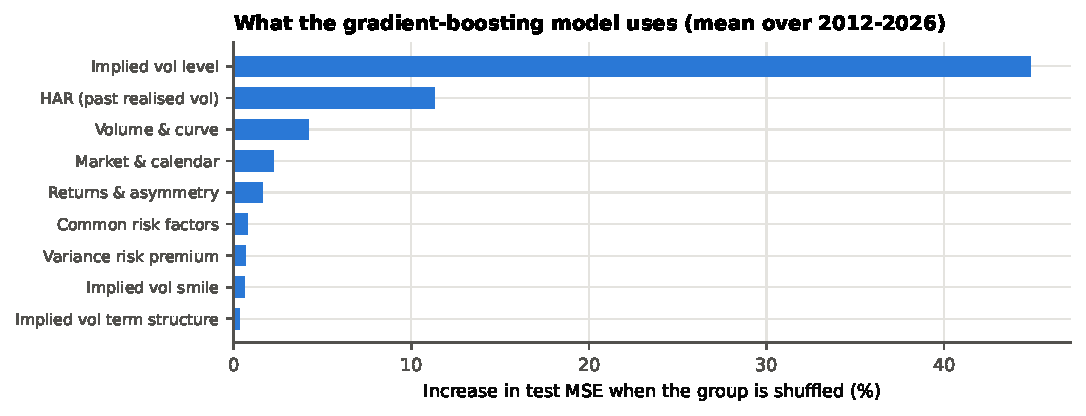
\includegraphics[width=0.9\textwidth]{v2_fig_importance.pdf}
\caption{Grouped permutation importance of gradient boosting on the test years: increase of test MSE when
all features of a group are shuffled together (mean over 2012--2026).}
\label{fig:importance}
\end{figure}

\subsection{Value for the haulier}

\begin{figure}[t]
\centering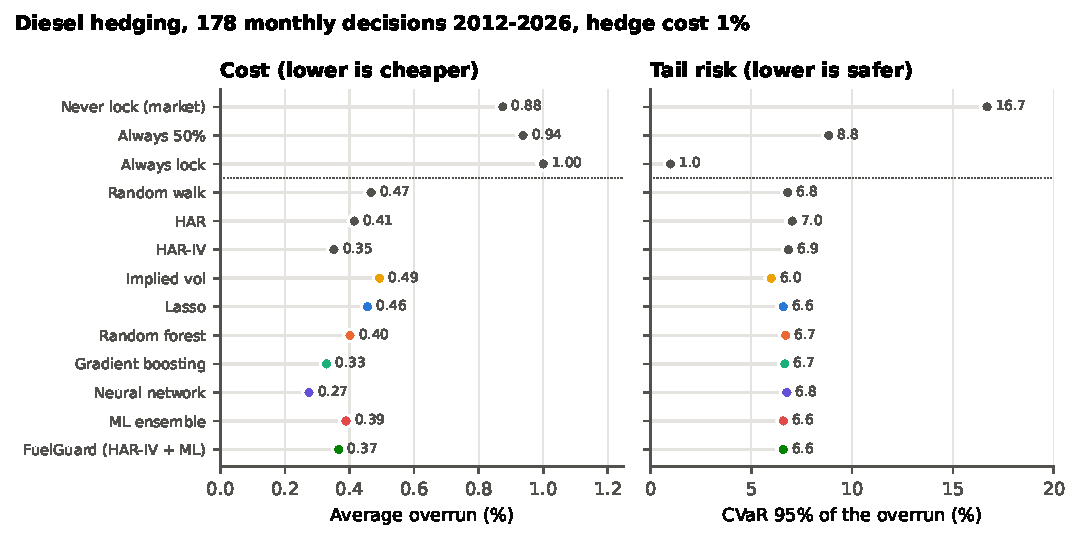
\includegraphics[width=\textwidth]{v2_fig_backtest.pdf}
\caption{Diesel hedging backtest. Each volatility forecast feeds the same rule (lock 100\% above the
historical 75th percentile of volatility, 50\% above the median). Overrun: monthly cost above the price
lockable at decision, with a 1\% hedging margin.}
\label{fig:backtest}
\end{figure}

\paragraph{Hedge ratio.} Figure~\ref{fig:backtest} and Table~\ref{tab:bt} (Appendix~\ref{app:additional})
evaluate 178 monthly decisions. Never hedging costs 0.88\% above the lockable price on average and 16.7\% in
the worst 5\% of months, about 2\,800~EUR more than the price that could have been fixed for our reference
firm. With FuelGuard, the firm hedges 40\% of months on average, its tail cost falls to \textbf{6.6\%}
(about 900~EUR) with only 8 months above a 5\% overrun instead of 38, and its average cost falls to 0.37\%,
saving about 900~EUR a year. A constant 50\% hedge achieves less (8.8\%) at a higher cost (0.94\%). The value
comes from \emph{conditioning the hedge on forecast risk}: all volatility forecasts, from the random walk to
FuelGuard, give tail costs between 6.0\% and 7.0\%, and the differences between them are within sampling
noise (the tail rests on 9 months).

\paragraph{95\% worst case.} The bound implied by FuelGuard's forecast averages 8.4\% above the lockable
price; it was exceeded in 14 of 178 months (7.9\% instead of 5\%; Kupiec $p=0.10$). All realised-volatility
models are slightly too optimistic (7--9\% breaches), because the Garman--Klass target ignores overnight
moves and the bound ignores fat tails; implied volatility, which includes the variance risk premium, has
correct coverage (5.6\%). A production version should scale the bound up by about 15\% or use implied
volatility as a floor.

\section{Limits and what we cannot claim}\label{sec:limits}

\begin{itemize}
\item \textbf{FuelGuard forecasts risk, not prices.} It cannot tell whether diesel will rise or fall; it
reduces the cost of bad months, it does not promise cheaper fuel on average (Appendix~\ref{app:v1}).
\item \textbf{The ML gain over the best benchmark is small.} 2.3\% across markets, significant; 0.7\% and
not significant for diesel. Most of the forecasting power comes from implied volatility, which the market
provides for free. Machine learning alone does not beat HAR-IV; it adds value in combination.
\item \textbf{Economic differences between forecasts are not significant.} In the hedging backtest, any
reasonable volatility forecast delivers most of the benefit; we cannot claim that FuelGuard's ranking above
HAR-IV in Figure~\ref{fig:backtest} would persist.
\item \textbf{Design choices after a first run.} The scale-free design and the combination were selected on
a 2010--2011 validation period after a first test run had shown raw ML losing to HAR-IV (Section~\ref{sec:methods}).
The validation period precedes every test year, but our first run had already seen the test years.
\item \textbf{Data.} US diesel futures, not ICE Gasoil; wholesale prices, so taxes (over half of the pump
price) and the basis to the haulier's supplier are ignored; overnight moves are missing from the realised
volatility target; the hedging margin is assumed (results are similar at 0\% and 2\%).
\item \textbf{Shocks from calm markets.} When a spike starts in a quiet market (2023, early 2026),
volatility forecasts react only after the first move.
\end{itemize}

\paragraph{With more time.} Use ICE Gasoil and a supplier price series; add intraday data for a full
realised variance; let the model learn the decision thresholds on validation data with a cost--CVaR
objective; forecast quantiles of the premium directly (quantile gradient boosting); calibrate the 95\%
bound; and add fundamentals (distillate inventories, refinery outages) and news indicators.

\section{Conclusion}

Machine learning could not predict the direction of diesel prices, and no honest product should claim it
can. It can, however, help forecast \emph{risk}. Pooling 22 futures markets with scale-free features and
combining the ML ensemble with the best econometric benchmark gives a small but statistically robust
improvement over HAR-IV, consistent across markets and years. For a small haulier, a hedge driven by forecast
volatility cuts the cost of the worst months by about 60\% at no extra average cost. The main lessons are
methodological: choose a target the data can predict, beat the right benchmark, pool data to give flexible
models enough observations, and choose designs on validation data, never on the test set.


\bibliographystyle{apalike}
\bibliography{references}

\clearpage
\appendix
\section{Machine-learning concepts used in the project}\label{app:theory}

\paragraph{A.1 Bias--variance trade-off.} For squared loss and $y=f(x)+\varepsilon$, the expected test
error of an estimator $\hat f$ trained on a random sample decomposes as
\[\E\big[(y-\hat f(x))^2\big]=\underbrace{\big(f(x)-\E\hat f(x)\big)^2}_{\text{bias}^2}+
\underbrace{\mathrm{Var}\big(\hat f(x)\big)}_{\text{variance}}+\sigma_\varepsilon^2 .\]
Flexible models (deep trees) have low bias and high variance; rigid models (penalised linear) the
opposite. The noise term $\sigma^2_\varepsilon$ is irreducible. In commodity markets it is very large
relative to the predictable part, so variance control (regularisation, averaging, small grids) matters more
than flexibility \citep[ch.~7]{hastie2009}.

\paragraph{A.2 Regularisation.} Ridge and $L_2$-logistic regression add $\lambda\lVert\beta\rVert_2^2$ to
the loss. In the linear case the solution $\hat\beta=(X^\top X+\lambda I)^{-1}X^\top y$ shrinks the
coefficients along the principal components of $X$, most strongly along low-variance directions, which
stabilises estimates when features are collinear. The penalty is not scale-invariant, so features are
standardised, using means and variances of the training window only.

\paragraph{A.3 Decision trees, bagging and random forests.} A CART tree chooses, at each node, the
feature and threshold that most reduce impurity (Gini or entropy for classification, squared error for
regression) and predicts the average outcome in each leaf. Trees are invariant to monotone transformations
of features and model interactions automatically, but small changes in the data change the tree a lot.
Bagging \citep{breiman1996} averages trees fitted on bootstrap samples; if each tree has variance $\sigma^2$
and pairwise correlation $\rho$, the average of $B$ trees has variance
$\rho\sigma^2+(1-\rho)\sigma^2/B$. As $B$ grows only $\rho\sigma^2$ remains, so random forests also
sample a subset of features at each split to decorrelate the trees \citep{breiman2001}. Because our labels
overlap in time, bootstrap samples contain near-duplicate rows; we subsample 50\% of rows per tree and use
large minimum leaf sizes to limit this (a ``sequential bootstrap'' as in \citealp{lopezdeprado2018} would
be a refinement).

\paragraph{A.4 Gradient boosting.} Boosting minimises $\sum_t L(y_t,F(x_t))$ by functional gradient
descent: starting from a constant $F_0$, at step $m$ compute pseudo-residuals
$r_{tm}=-\partial L(y_t,F)/\partial F|_{F=F_{m-1}(x_t)}$, fit a small regression tree $h_m$ to them, and update
$F_m=F_{m-1}+\nu h_m$ \citep{friedman2001}. For the log loss on the log-odds scale, $r_{tm}=y_t-\hat\pi_{m-1}(x_t)$.
A small learning rate $\nu$ with more trees acts as regularisation (shrinkage); the depth of the trees
bounds the order of interactions.

\paragraph{A.5 Proper scoring rules and probability evaluation.} A scoring rule $S(p,y)$ is strictly
proper if $\E_{y\sim q}S(p,y)$ is uniquely optimised at $p=q$ \citep{gneiting2007}. The log loss and the
Brier score $(p-y)^2$ are both strictly proper, so they reward honest probabilities; accuracy is not.
The Brier skill score $1-\mathrm{BS}/\mathrm{BS}_{\text{ref}}$ compares a model with the climatological
forecast (the training base rate): positive values mean the model adds information. The ROC AUC equals the
probability that a randomly chosen spike day receives a higher score than a randomly chosen non-spike day
\citep{fawcett2006}; it measures ranking (discrimination) and ignores calibration, which is shown
separately with a reliability diagram.

\paragraph{A.6 Cross-validation for overlapping financial labels.} Standard $K$-fold CV assumes
independent observations. With time series, a random split puts tomorrow's data in the training set and
yesterday's in the validation set; with \emph{overlapping} labels (each label uses the next 22 days) even a
chronological split leaks, because the last training labels are computed from prices inside the validation
period. \emph{Purging} removes every training row whose label window ends after the validation period
starts; an \emph{embargo} removes a further block of rows, because features are also autocorrelated
\citep[ch.~7]{lopezdeprado2018}. We apply both in the outer walk-forward loop and in the inner
cross-validation used to tune hyper-parameters, and test them automatically (\texttt{tests/test\_leakage.py}).

\paragraph{A.7 Permutation importance.} The importance of feature $j$ is the drop in out-of-sample
performance (here AUC) when column $j$ of the test set is randomly permuted, which breaks its link with the
target while keeping its distribution \citep{fisher2019}. Unlike impurity-based importance it is computed
on test data and is not biased towards high-cardinality features \citep{strobl2007}. With correlated
features it understates the importance of each member of a correlated group, so we also report importance
summed by group.

\paragraph{A.8 Diebold--Mariano test.} To compare two forecasts with errors $e_{1t},e_{2t}$, define
$d_t=e_{1t}^2-e_{2t}^2$. Under the null of equal accuracy $\E d_t=0$, and
$\mathrm{DM}=\bar d/\sqrt{\widehat{\mathrm{LRV}}(d)/n}\to\mathcal N(0,1)$ \citep{diebold1995}. Daily forecasts of a
21-day average are autocorrelated by construction, so the long-run variance uses a Newey--West estimator
with 21 lags \citep{newey1987}.

\paragraph{A.9 Conditional Value-at-Risk.} For a loss $X$, $\mathrm{CVaR}_{95}(X)=\E[X\mid X\ge
\mathrm{VaR}_{95}(X)]$, the average of the worst 5\% outcomes \citep{rockafellar2000}. Unlike variance, it
only penalises bad outcomes, which matches the haulier's concern: months when diesel costs far more than
the price that could have been locked.

\paragraph{A.10 Realised volatility and the Garman--Klass estimator.} Volatility is not observed; it is
estimated from prices. Squared daily returns are unbiased but very noisy, and with generic futures series
they are contaminated by contract rolls. Range-based estimators use the open $O$, high $H$, low $L$ and close
$C$ of the same contract on the same day. \citet{garman1980} show that
$\hat\sigma^2_{GK}=\tfrac12\ln^2(H/L)-(2\ln2-1)\ln^2(C/O)$ is unbiased under a driftless random walk and up to
seven times more efficient than the squared close-to-close return. Averaging it over 21 days gives our
realised-volatility target. It ignores overnight moves, which are small for futures that trade almost 24
hours, larger for agricultural contracts.

\paragraph{A.11 The HAR model.} \citet{corsi2009} models tomorrow's (log) realised volatility as a linear
function of its daily, weekly and monthly averages,
$\ln\sigma_{t+1:t+h}=\beta_0+\beta_d\ln\sigma_t^{(1)}+\beta_w\ln\sigma_t^{(5)}+\beta_m\ln\sigma_t^{(22)}+\varepsilon$.
The cascade reproduces the long memory of volatility with three parameters, and it is the standard
benchmark that machine-learning volatility models must beat \citep{christensen2023}. Adding the log implied
volatility (HAR-IV) brings in the market's forward-looking forecast; implied volatility exceeds
subsequent realised volatility on average (the variance risk premium) but contains information not in past
returns \citep{bollerslev2009}.

\paragraph{A.12 Neural networks.} The multilayer perceptron computes
$f(x)=W_3\,\phi(W_2\,\phi(W_1x+b_1)+b_2)+b_3$ with ReLU activations $\phi(z)=\max(0,z)$; with enough units it
can approximate any continuous function. It is trained by stochastic gradient descent (Adam) on the squared
loss with an $L_2$ penalty $\alpha$ on the weights, and with \emph{early stopping}: 10\% of the training rows
are held out and training stops when their loss no longer improves, a form of regularisation. Inputs must be
standardised. Neural networks need many observations; pooling 22 markets is what makes them usable here
\citep{gu2020}.

\paragraph{A.13 Lasso.} The Lasso adds $\alpha\lVert\beta\rVert_1$ to the squared loss. Unlike ridge, the
$L_1$ penalty sets some coefficients exactly to zero (the solution sits on a corner of the constraint set), so
it performs variable selection; with correlated features it tends to keep one member of a group.

\paragraph{A.14 Forecast combination.} Averaging forecasts of different models reduces variance when their
errors are imperfectly correlated, by the same argument as bagging (A.3). Equal weights are hard to beat
because estimated weights add noise; our ``ML ensemble'' is the simple mean of the four ML forecasts, fixed
in advance.

\paragraph{A.15 Loss functions for volatility and coverage tests.} Realised volatility is a noisy proxy
of true volatility. \citet{patton2011} shows that only some loss functions rank forecasts consistently when
the proxy is noisy: the squared error and the QLIKE loss $\hat\sigma^{-2}\sigma^2-\ln(\hat\sigma^{-2}\sigma^2)-1$,
which penalises under-prediction of risk more than over-prediction. For the 95\% cost bound we use the
\citet{kupiec1995} test: with $x$ breaches in $N$ months, $\mathrm{LR}=-2\ln\frac{0.95^{N-x}0.05^{x}}
{(1-\hat p)^{N-x}\hat p^{x}}\sim\chi^2_1$ under correct coverage, $\hat p=x/N$.

\section{Data dictionary}\label{app:data}

\begin{sloppypar}
\paragraph{Futures panel (FuelGuard 2.0).} Source: Bloomberg terminal, \texttt{BDH} formulas, downloaded
17--19 November 2026. Fields per market: \texttt{PX\_SETTLE}, \texttt{PX\_OPEN}, \texttt{PX\_HIGH},
\texttt{PX\_LOW}, \texttt{PX\_VOLUME} of the first generic contract, \texttt{PX\_SETTLE} of the second, and
\texttt{30DAY\_IMPVOL\_x\%MNY\_DF} for $x\in\{90,95,97.5,100,102.5,105,110\}$ plus
\texttt{1ST\_MTH\_IMPVOL\_100.0\%MNY\_DF} and \texttt{2ND\_MTH\_IMPVOL\_100.0\%MNY\_DF}. Common series:
VIX, VIX3M (\texttt{PX\_LAST}) and VSTOXX (V2X).
\end{sloppypar}

\begin{table}[H]
\centering\scriptsize
\fittable{\tabdir/vol_markets.tex}
\caption{The 22 markets: market-days with a target, median and 95th percentile of realised volatility
(Garman--Klass, next 21 days, annualised) and median 30-day implied volatility. Government-bond volatilities
are price volatilities.}
\label{tab:markets}
\end{table}

\paragraph{Diesel cost series (FuelGuard 1.0 and backtest).} The 21 daily series of Appendix~\ref{app:v1}
(Table~\ref{tab:v1raw}) and the ECB euro reference rate (USD per EUR), used to express diesel in EUR/litre
(1 gallon = 3.785 litres).

\begin{table}[H]
\centering\scriptsize
\fittable{\tabdir/descriptive_raw.tex}
\caption{Raw series of FuelGuard 1.0 and the derived diesel price.}
\label{tab:v1raw}
\end{table}

\section{Additional results}\label{app:additional}

\begin{table}[H]
\centering\small
\fittable{\tabdir/vol_validation_design.tex}
\caption{Design selection on the validation period 2010--2011 (training labels known before December 2009;
11\,115 market-days). ``vs HAR-IV'': MSE reduction relative to HAR-IV. The last row is the design used in
the walk-forward.}
\label{tab:design}
\end{table}

\begin{table}[H]
\centering\small
\fittable{\tabdir/vol_by_market.tex}
\caption{By market, 2012--2026: $R^2$ of HAR-IV and FuelGuard within each market, MSE reduction and DM
statistic of FuelGuard against HAR-IV (Newey--West, 21 lags; $<-1.96$: significantly better), and the best
single ML model.}
\end{table}

\begin{figure}[H]
\centering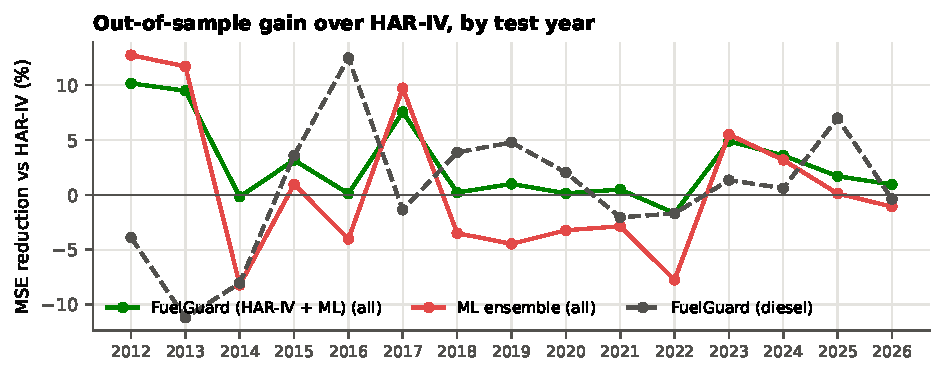
\includegraphics[width=0.95\textwidth]{v2_fig_by_year.pdf}
\caption{MSE reduction against HAR-IV by test year.}
\end{figure}

\begin{table}[H]
\centering\small
\fittable{\tabdir/vol_backtest.tex}
\caption{Diesel hedging backtest, 178 monthly decisions 2012--2026, hedge cost 1\%. Mean, St.dev, CVaR95
and Worst refer to the overrun of the monthly cost over the lockable price; EUR figures for 25\,000
litres a month.}
\label{tab:bt}
\end{table}

\begin{table}[H]
\centering\small
\fittable{\tabdir/vol_var_coverage.tex}
\caption{95\% worst-case bound: breaches over 178 monthly decisions (5\% expected), Kupiec test, average
bound, and breach rate over all daily decisions (overlapping windows).}
\end{table}

\begin{table}[H]
\centering\small
\fittable{\tabdir/vol_hyperparameters.tex}
\caption{Most frequent hyper-parameters chosen by purged cross-validation across the 15 training windows.}
\end{table}

\section{First attempt: predicting price spikes (FuelGuard 1.0)}\label{app:v1}

Our first design asked machine learning to predict the \emph{price} directly. It is reported here because
its failure motivated the final product, and because the guidelines ask what the product cannot do.

\paragraph{Set-up.} Daily decisions on NYMEX diesel trading days, January 2008 -- October 2026 (4\,701
days), 21 raw series (diesel, Brent, WTI and gas futures for two maturities; diesel and Brent implied
volatility; copper, gold, 10-year Treasury futures; VIX and VIX3M; S\&P~500 and energy indices; US and euro
inflation expectations; ECB EUR/USD) and 57 engineered features. A decision at the close of $t$ is executed
at the settlement of $t+1$. The \emph{market cost} $M_t$ is the average diesel price in EUR/litre over
$t+2,\dots,t+22$; the \emph{lockable price} $P_t$ is a strip of first- and second-month futures settled at
$t+1$, each day priced with the contract that will be front month on that day (generic contracts roll on
the first trading day of the month; comparing different delivery months would create a spurious gain from
locking, a mistake our very first analysis made). Targets: the premium $R_t=M_t/P_t-1$ (regression) and a
\emph{spike} $\1\{R_t>5\%\}$ (classification, 19\% of days). Models: $L_2$-logistic and ridge, random forest,
gradient boosting, in the same purged expanding walk-forward (2012--2026). These $M_t$ and $P_t$ are reused
by the FuelGuard~2.0 backtest.

\paragraph{Results.} The premium was not predictable: the best out-of-sample $R^2$ against the futures price
was 0.5\%, no Diebold--Mariano test was significant, and cross-validation always chose the strongest ridge
penalty, i.e.\ a constant. Spikes were predictable only modestly (Table~\ref{tab:v1}): AUC 0.59--0.64 for the
57-feature models, positive Brier skill only for the random forest, while ranking days by diesel implied
volatility alone gave an AUC of 0.71. Skill collapsed in 2023 and 2026, when spikes started from calm
markets. In the hedging backtest a simple rule ``lock when implied volatility is above its median''
beat every classifier. The lesson: the predictable part of the problem is \emph{volatility}, not direction,
which led to FuelGuard~2.0.

\begin{table}[H]
\centering\small
\fittable{\tabdir/classification_oos.tex}
\caption{FuelGuard 1.0, spike classification out of sample 2012--2026 (3\,725 days). The one-feature
implied-volatility logistic was added after a first run. Last row: days ranked by implied volatility, no model.}
\label{tab:v1}
\end{table}

\section{Contribution statement}\label{app:contribution}

\emph{To be completed and signed by the five members before submission.}

\begin{center}
\renewcommand{\arraystretch}{1.6}
\begin{tabular}{p{3.2cm}p{8.2cm}p{3.2cm}}
\toprule
\textbf{Member} & \textbf{Main contributions} & \textbf{Signature}\\
\midrule
{[Member 1]} & e.g.\ Bloomberg download, data dictionary, data preparation & \\
{[Member 2]} & e.g.\ feature engineering, leakage tests & \\
{[Member 3]} & e.g.\ models, walk-forward evaluation, hyper-parameter tuning & \\
{[Member 4]} & e.g.\ hedging backtest, report sections 1, 5, 6; quant deck & \\
{[Member 5]} & e.g.\ client research, sales deck, report sections 1--2, editing & \\
\bottomrule
\end{tabular}
\end{center}
All members read the full report and can explain the intuition of every method used.

\section{Use of AI tools}\label{app:ai}

\emph{The group should complete this section with its own account; the draft below describes how the
AI assistant was used to produce the first version of the repository and report.}

\paragraph{Tool.} Claude (Anthropic), used through the Claude app.

\paragraph{Tasks.}
\begin{itemize}
\item \textbf{Brainstorming the product}: from an initial idea on electricity costs for Italian SMEs to
the final diesel-hedging product, choice of client (bank) and benchmark.
\item \textbf{Data}: list of Bloomberg tickers and fields; parsing of the Bloomberg Excel exports and of
the ECB SDMX file.
\item \textbf{Code}: first version of the full pipeline (\texttt{src/fuelguard}, \texttt{scripts/}),
including the purged walk-forward evaluation and the leakage tests.
\item \textbf{Report}: first draft of the text, figures and tables, including Appendix~\ref{app:theory}.
\end{itemize}

\paragraph{Main prompts (abridged).} ``Which data can we use to build a small university project to
automate hedging of energy costs for SMEs in Italy with machine learning?''; ``Can we simplify it using oil?
Focus on a specific subtopic: what are we selling?''; ``Are these Bloomberg files enough to do a first
analysis?''; ``Which directions do you propose if results are not good?''; ``Build a full GitHub repository
with a paper, fully analysed, including the theoretical concepts of machine learning.''; ``It does not work
well, confirm? Let's find a way to make machine learning work: change the objective or the system, reason
first about what could work, inspired by the literature.''; ``Redo it on volatility.''

\paragraph{How we checked the outputs.} [To be completed by the group, e.g.:] we reran the full pipeline
from a clean copy; checked the leakage tests and added a deliberately leaky feature to verify that the test
fails; compared yearly average prices with published figures; recomputed key numbers of Section~\ref{sec:results}
from the saved predictions; checked every reference; and rewrote the sections we present.
Corrections made during the work: a first analysis compared futures of different delivery months and
overstated the benefit of always locking (fixed with a same-contract strip, Appendix~\ref{app:v1}); the
spike-prediction product was replaced by volatility forecasting after it failed out of sample; and the
final ML design was chosen on a 2010--2011 validation period rather than on the test years
(Section~\ref{sec:methods}).

\end{document}
